\documentclass[11pt,a4paper]{article}

%\usepackage[T1]{fontenc}
\usepackage[utf8]{inputenc}
%\usepackage{lmodern}
\usepackage{amsmath,amssymb}
\usepackage{siunitx}
\usepackage{graphicx}
\usepackage{booktabs}
\usepackage{tikz}
\usepackage{pgfplots}
\usepackage[margin=25mm]{geometry}
\usepackage{hyperref}
\usepackage{caption}

\pgfplotsset{compat=1.16}
\usetikzlibrary{arrows.meta,patterns,calc}

\sisetup{output-decimal-marker={,},per-mode=symbol,range-phrase={~a~},range-units=single}

% localizzazione minima (babel-italian non disponibile in questa installazione)
\renewcommand{\contentsname}{Indice}
\renewcommand{\refname}{Riferimenti bibliografici}
\renewcommand{\figurename}{Fig.}
\renewcommand{\tablename}{Tab.}
\renewcommand{\abstractname}{Sommario}

\hypersetup{colorlinks=true,linkcolor=black,citecolor=black,urlcolor=blue}

\title{Il \emph{power diode} a giunzione PIN\\
\large Fisica dei portatori, livelli di Fermi, conduzione diretta e \emph{reverse recovery}}
\author{}
\date{}

\begin{document}
\maketitle

\begin{abstract}
\noindent
Questa nota descrive il funzionamento del \emph{power diode} a struttura PIN
($p^{+}$--$n^{-}$--$n^{+}$), utilizzato come \emph{freewheeling diode},
\emph{clamping diode} e raddrizzatore nei convertitori di potenza. Si parte dal
diagramma a bande e dai livelli di Fermi, si analizza la distribuzione dei
portatori in conduzione diretta (\emph{high-level injection} e
\emph{conductivity modulation}), si descrive in dettaglio il fenomeno di
\emph{reverse recovery} con le relative grandezze di datasheet, e si chiude con
le tecniche costruttive (\emph{lifetime control}, \emph{emitter efficiency
control}, MPS) e con l'impatto a livello di convertitore.
\end{abstract}

\tableofcontents
\bigskip

%======================================================================
\section{Perché una struttura PIN}
%======================================================================

Un diodo di segnale è una semplice giunzione $p$--$n$ con entrambe le regioni
fortemente drogate. Per tenere una tensione inversa elevata questa struttura non
è utilizzabile: il campo elettrico di picco raggiungerebbe il valore critico
$E_c$ su una distanza troppo breve.

Nella struttura PIN si interpone quindi fra i due \emph{emitter} una regione
debolmente drogata, la \emph{drift region} (o \emph{base region}) $n^{-}$, che
sostiene la tensione inversa. Nel caso \emph{non-punch-through} (NPT) la
distribuzione di campo è triangolare e valgono

\begin{equation}
V_{BR} = \frac{\varepsilon_{Si} E_c^{2}}{2 q N_D},
\qquad
W_{D} = \frac{2 V_{BR}}{E_c} = \sqrt{\frac{2 \varepsilon_{Si} V_{BR}}{q N_D}} ,
\end{equation}

con $E_c \approx \SI{2e5}{\volt\per\centi\meter}$ nel silicio (dipendente da
$N_D$). Nel caso \emph{punch-through} (PT), con \emph{buffer layer} $n$ fra
\emph{drift region} e $n^{+}$, il campo è trapezoidale e a parità di $V_{BR}$ la
regione può essere più sottile di circa il \SI{30}{\percent}:

\begin{equation}
V_{BR} = E_c W_{D} - \frac{q N_D W_{D}^{2}}{2 \varepsilon_{Si}} .
\end{equation}

Come ordine di grandezza, per un diodo da \SI{1700}{\volt} servono
$W_D \approx \SIrange{200}{250}{\micro\meter}$ con
$N_D \approx \SI{1e14}{\per\centi\meter\cubed}$.

\begin{figure}[htbp]
\centering
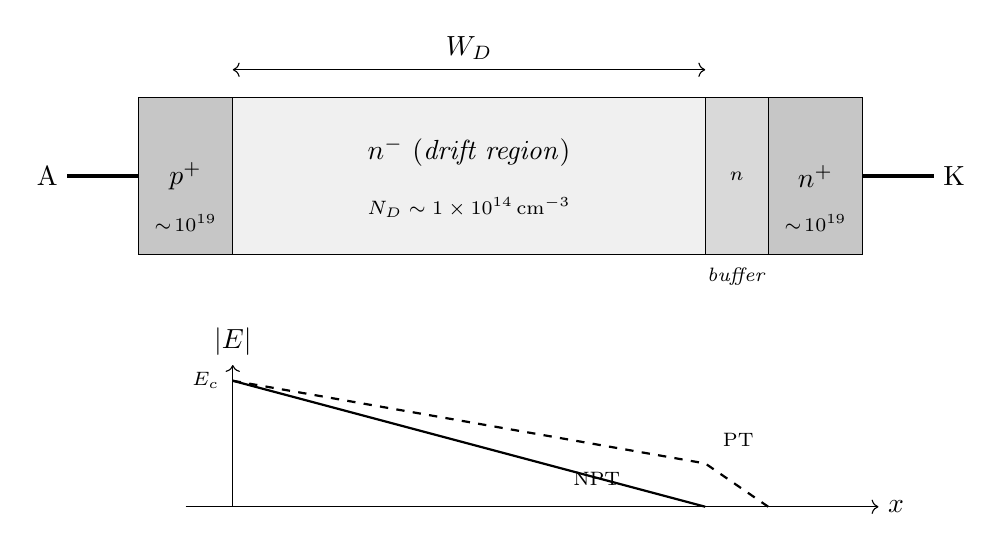
\begin{tikzpicture}[scale=1.0]
% strati
\fill[gray!45] (0,0) rectangle (1.2,2);
\fill[gray!12] (1.2,0) rectangle (7.2,2);
\fill[gray!30] (7.2,0) rectangle (8.0,2);
\fill[gray!45] (8.0,0) rectangle (9.2,2);
\draw (0,0) rectangle (9.2,2);
\draw (1.2,0) -- (1.2,2);
\draw (7.2,0) -- (7.2,2);
\draw (8.0,0) -- (8.0,2);
\node at (0.6,1.0) {$p^{+}$};
\node at (4.2,1.3) {$n^{-}$ (\emph{drift region})};
\node at (7.6,1.0) {\scriptsize $n$};
\node at (8.6,1.0) {$n^{+}$};
\node at (4.2,0.6) {\scriptsize $N_D \sim \SI{1e14}{\per\centi\meter\cubed}$};
\node at (0.6,0.4) {\scriptsize $\sim\!10^{19}$};
\node at (8.6,0.4) {\scriptsize $\sim\!10^{19}$};
\node[below] at (7.6,-0.05) {\scriptsize \emph{buffer}};
% terminali
\draw[very thick] (-0.9,1.0) -- (0,1.0);
\draw[very thick] (9.2,1.0) -- (10.1,1.0);
\node[left] at (-0.9,1.0) {A};
\node[right] at (10.1,1.0) {K};
% quote
\draw[<->] (1.2,2.35) -- (7.2,2.35) node[midway,above] {$W_D$};
% campo elettrico
\begin{scope}[yshift=-3.2cm]
  \draw[->] (1.2,0) -- (1.2,1.8) node[above] {$|E|$};
  \draw[->] (0.6,0) -- (9.4,0) node[right] {$x$};
  \draw[thick] (1.2,1.6) -- (7.2,0.0);
  \draw[thick,dashed] (1.2,1.6) -- (7.2,0.55) -- (8.0,0.0);
  \node[right] at (7.3,0.85) {\scriptsize PT};
  \node[right] at (5.4,0.35) {\scriptsize NPT};
  \node[left] at (1.15,1.6) {\scriptsize $E_c$};
\end{scope}
\end{tikzpicture}
\caption{Struttura del \emph{power diode} PIN e profilo del campo elettrico in
blocco inverso: triangolare nel caso NPT, trapezoidale nel caso PT con
\emph{buffer layer} (o \emph{field stop}).}
\end{figure}

Il problema della struttura PIN è che la \emph{drift region}, così debolmente
drogata, avrebbe in condizioni ohmiche una resistenza specifica proibitiva:

\begin{equation}
R_{on,sp} = \frac{W_D}{q \mu_n N_D} .
\end{equation}

Per $W_D = \SI{250}{\micro\meter}$ e $N_D = \SI{1e14}{\per\centi\meter\cubed}$
si otterrebbero decine di \si{\ohm\centi\meter\squared}, cioè caduta di decine
di volt a densità di corrente tipiche. Il funzionamento reale è possibile solo
grazie alla \emph{conductivity modulation}: in conduzione la regione viene
inondata di un plasma elettroni--lacune con concentrazioni di 2--3 ordini di
grandezza superiori a $N_D$. Questo è il compromesso fondamentale del diodo
bipolare: bassa $V_F$ in conduzione, ma carica immagazzinata da rimuovere allo
spegnimento (\emph{reverse recovery}).

%======================================================================
\section{Bande di energia e livelli di Fermi}
%======================================================================

\subsection{Equilibrio termodinamico}

In equilibrio (nessuna polarizzazione, nessuna corrente) il livello di Fermi
$E_F$ è \emph{costante} in tutta la struttura. È questa condizione che impone la
curvatura delle bande (\emph{band bending}) alla giunzione: nella regione $p^{+}$
$E_F$ è vicino a $E_V$, nella regione $n$ è vicino a $E_C$, e per allineare
$E_F$ le bande devono spostarsi della quantità $qV_{bi}$.

Con statistica di Boltzmann:

\begin{equation}
n = n_i \exp\!\left(\frac{E_F - E_i}{kT}\right),
\qquad
p = n_i \exp\!\left(\frac{E_i - E_F}{kT}\right),
\qquad
np = n_i^{2} .
\end{equation}

Il \emph{built-in potential} vale

\begin{equation}
V_{bi} = \frac{kT}{q} \ln\!\left(\frac{N_A N_D}{n_i^{2}}\right)
\approx \SIrange{0.7}{0.9}{\volt} \ \text{nel silicio}.
\end{equation}

Si noti che $V_{bi}$ non è una tensione misurabile ai morsetti: le cadute di
contatto la compensano esattamente, altrimenti si avrebbe corrente a
circuito chiuso senza generatore.

\subsection{Quasi-Fermi levels in polarizzazione}

Fuori equilibrio il concetto di livello di Fermi unico perde significato e si
introducono i due \emph{quasi-Fermi levels} (o \emph{imref}) $E_{Fn}$ ed
$E_{Fp}$:

\begin{equation}
n = n_i \exp\!\left(\frac{E_{Fn} - E_i}{kT}\right),
\qquad
p = n_i \exp\!\left(\frac{E_i - E_{Fp}}{kT}\right),
\end{equation}

da cui la relazione chiave

\begin{equation}
\boxed{\; np = n_i^{2} \exp\!\left(\frac{E_{Fn} - E_{Fp}}{kT}\right)
= n_i^{2} \exp\!\left(\frac{qV_{j}}{kT}\right) \;}
\label{eq:splitting}
\end{equation}

dove $V_j$ è la tensione applicata alla giunzione. Lo \emph{splitting} dei due
quasi-livelli \emph{è} la polarizzazione, espressa in energia.

Le densità di corrente si scrivono in forma compatta come gradienti dei
quasi-Fermi levels, il che unifica drift e diffusione:

\begin{equation}
J_n = \mu_n n \, \frac{d E_{Fn}}{dx},
\qquad
J_p = \mu_p p \, \frac{d E_{Fp}}{dx} .
\end{equation}

Di qui una lettura immediata: \emph{dove un quasi-Fermi level è piatto, la
corrispondente componente di corrente è nulla}.

\begin{itemize}
\item \textbf{Forward bias.} $E_{Fn}$ ed $E_{Fp}$ si separano di $qV_j$ alla
giunzione $p^{+}n^{-}$; nella \emph{drift region} in \emph{high-level injection}
entrambi sono spinti dentro (o vicinissimo a) le bande, e la loro pendenza
residua rende conto della caduta ohmica sul plasma. Il prodotto $np \gg n_i^2$.
\item \textbf{Reverse bias.} La separazione si inverte
($E_{Fn} - E_{Fp} = qV_j < 0$), quindi $np \ll n_i^{2}$: nella \emph{space
charge region} prevale la generazione termica, che dà la corrente di leakage
$J_{gen} = q n_i W_{scr} / \tau_g$, fortemente dipendente dalla temperatura.
\item \textbf{Equilibrio.} $E_{Fn} = E_{Fp} = E_F$, e la \eqref{eq:splitting} si
riduce a $np = n_i^2$.
\end{itemize}

\begin{figure}[htbp]
\centering
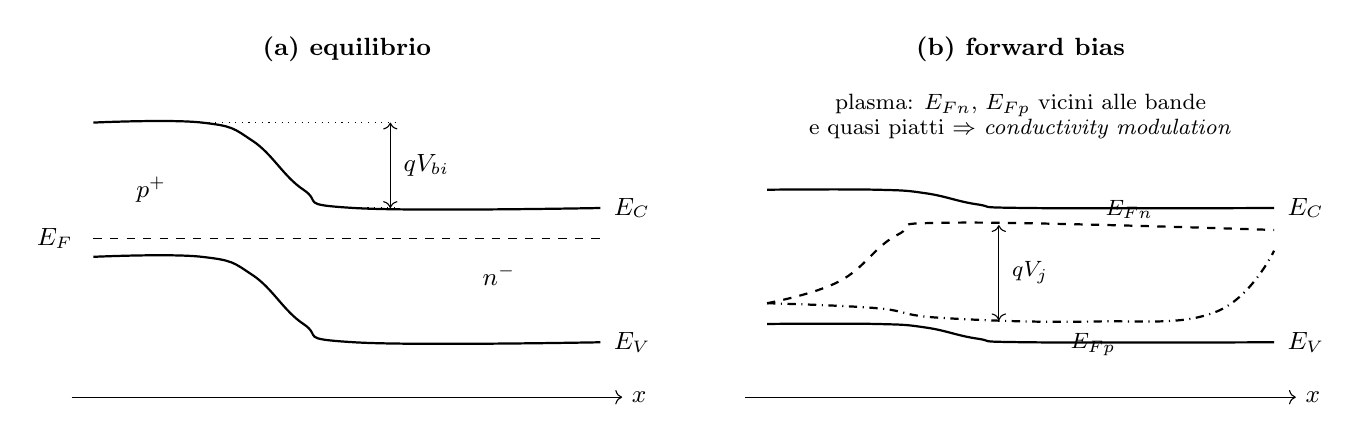
\begin{tikzpicture}[xscale=0.92,yscale=1.55,font=\small]
% ================= (a) equilibrio =================
\begin{scope}
  \draw[->] (-0.3,-0.75) -- (7.3,-0.75) node[right] {$x$};
  \draw[thick] plot[smooth,tension=0.7] coordinates
    {(0,1.5) (1.5,1.5) (2.2,1.35) (2.9,0.95) (3.6,0.80) (7,0.80)};
  \draw[thick] plot[smooth,tension=0.7] coordinates
    {(0,0.40) (1.5,0.40) (2.2,0.25) (2.9,-0.15) (3.6,-0.30) (7,-0.30)};
  \draw[dashed] (0,0.55) -- (7,0.55);
  \node[right] at (7.05,0.80) {$E_C$};
  \node[right] at (7.05,-0.30) {$E_V$};
  \node[left] at (-0.15,0.55) {$E_F$};
  \node at (0.8,0.95) {$p^{+}$};
  \node at (5.6,0.25) {$n^{-}$};
  \draw[dotted] (1.5,1.5) -- (4.2,1.5);
  \draw[dotted] (3.6,0.80) -- (4.2,0.80);
  \draw[<->] (4.1,1.5) -- (4.1,0.80);
  \node[right] at (4.15,1.15) {$qV_{bi}$};
  \node at (3.5,2.1) {\textbf{(a) equilibrio}};
\end{scope}
% ================= (b) forward bias =================
\begin{scope}[xshift=9.3cm]
  \draw[->] (-0.3,-0.75) -- (7.3,-0.75) node[right] {$x$};
  \draw[thick] plot[smooth,tension=0.7] coordinates
    {(0,0.95) (1.5,0.95) (2.2,0.92) (2.9,0.83) (3.6,0.80) (7,0.80)};
  \draw[thick] plot[smooth,tension=0.7] coordinates
    {(0,-0.15) (1.5,-0.15) (2.2,-0.18) (2.9,-0.27) (3.6,-0.30) (7,-0.30)};
  % quasi-Fermi levels
  \draw[dashed,thick] plot[smooth,tension=0.7] coordinates
    {(0,0.02) (1.0,0.20) (1.8,0.58) (2.6,0.68) (7,0.62)};
  \draw[dash dot,thick] plot[smooth,tension=0.7] coordinates
    {(0,0.02) (1.5,-0.02) (2.4,-0.10) (4.5,-0.13) (6.2,-0.05) (7,0.45)};
  \node[right] at (7.05,0.80) {$E_C$};
  \node[right] at (7.05,-0.30) {$E_V$};
  \node[above] at (5.0,0.63) {\footnotesize $E_{Fn}$};
  \node[below] at (4.5,-0.15) {\footnotesize $E_{Fp}$};
  \draw[<->] (3.2,0.66) -- (3.2,-0.12);
  \node[right] at (3.25,0.27) {\footnotesize $qV_j$};
  \node at (3.5,2.1) {\textbf{(b) forward bias}};
  \node[align=center] at (3.5,1.55)
    {\footnotesize plasma: $E_{Fn}$, $E_{Fp}$ vicini alle bande\\[-2pt]
     \footnotesize e quasi piatti $\Rightarrow$ \emph{conductivity modulation}};
\end{scope}
\end{tikzpicture}
\caption{Diagramma a bande della giunzione $p^{+}n^{-}$. (a) In equilibrio
$E_F$ è unico e piatto, le bande si curvano di $qV_{bi}$. (b) In
\emph{forward bias} la barriera si riduce e i due \emph{quasi-Fermi levels} si
separano di $qV_j$; nella \emph{drift region} in alta iniezione sono
quasi piatti e spinti verso i bordi banda. Ai contatti ohmici i due livelli
tornano a coincidere.}
\end{figure}

%======================================================================
\section{Conduzione diretta}
%======================================================================

\subsection{Bassa iniezione: il modello di Shockley}

A correnti molto basse ($n \ll N_D$) vale la relazione ideale

\begin{equation}
J = J_S \left[ \exp\!\left(\frac{qV}{n_{id} kT}\right) - 1 \right],
\qquad
J_S = q n_i^{2}\left(\frac{D_p}{L_p N_D} + \frac{D_n}{L_n N_A}\right),
\end{equation}

con $n_{id}=1$ per corrente di diffusione e $n_{id}=2$ quando domina la
ricombinazione nella \emph{space charge region} (regime tipico a bassissima
corrente).

\subsection{Alta iniezione: plasma e conductivity modulation}

Alle densità di corrente d'impiego ($\SIrange{50}{200}{\ampere\per\centi\meter\squared}$)
il diodo di potenza lavora sempre in \emph{high-level injection}: entrambi gli
\emph{emitter} iniettano nella \emph{drift region} e vale

\begin{equation}
n(x) \simeq p(x) \gg N_D \qquad (\text{tipicamente } 10^{16}\!-\!10^{17}\ \si{\per\centi\meter\cubed}).
\end{equation}

La neutralità di carica lega i due profili, e il trasporto è descritto
dall'\emph{ambipolar diffusion equation}:

\begin{equation}
\frac{\partial n}{\partial t}
= D_a \frac{\partial^{2} n}{\partial x^{2}} - \frac{n}{\tau_{HL}},
\qquad
D_a = \frac{2 D_n D_p}{D_n + D_p},
\qquad
L_a = \sqrt{D_a \tau_{HL}} .
\end{equation}

Nel silicio $D_a \approx \SI{18}{\centi\meter\squared\per\second}$. Il termine
di \emph{drift} scompare formalmente perché in alta iniezione il campo si
autoregola per mantenere uguali i flussi delle due specie: da qui il nome
\emph{ambipolare}.

In regime stazionario, con $d = W_D/2$ e le condizioni al contorno date dalle
correnti ai due \emph{emitter}, si ottiene la classica soluzione a \emph{catenaria}
(Hall):

\begin{equation}
n(x) = \frac{\tau_{HL} I_F}{2 q A L_a}
\left[
\frac{\cosh(x/L_a)}{\sinh(d/L_a)}
- \frac{\mu_n - \mu_p}{\mu_n + \mu_p}\,
\frac{\sinh(x/L_a)}{\cosh(d/L_a)}
\right] .
\label{eq:catenaria}
\end{equation}

\begin{figure}[htbp]
\centering
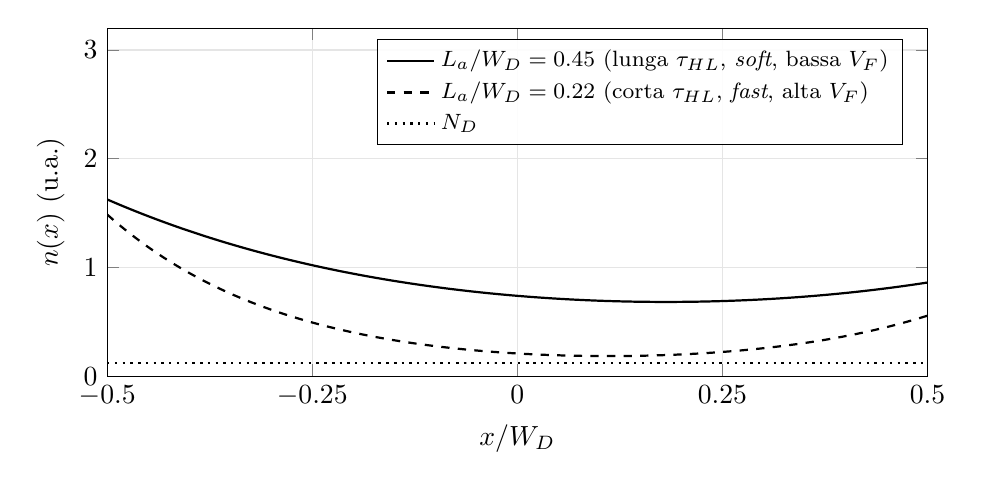
\begin{tikzpicture}
\begin{axis}[
  width=12cm, height=6cm,
  xlabel={$x/W_D$}, ylabel={$n(x)$ (u.a.)},
  xmin=-0.5, xmax=0.5, ymin=0, ymax=3.2,
  xtick={-0.5,-0.25,0,0.25,0.5},
  legend pos=north east, legend cell align=left,
  legend style={font=\footnotesize,fill=white,fill opacity=0.9,text opacity=1},
  grid=both, grid style={gray!20},
  samples=200,
]
\addplot[thick,domain=-0.5:0.5]
  { (exp(x/0.45)+exp(-x/0.45))/(exp(0.5/0.45)-exp(-0.5/0.45))
    - 0.475*(exp(x/0.45)-exp(-x/0.45))/(exp(0.5/0.45)+exp(-0.5/0.45)) };
\addlegendentry{$L_a/W_D = 0.45$ (lunga $\tau_{HL}$, \emph{soft}, bassa $V_F$)}
\addplot[thick,dashed,domain=-0.5:0.5]
  { (exp(x/0.22)+exp(-x/0.22))/(exp(0.5/0.22)-exp(-0.5/0.22))
    - 0.475*(exp(x/0.22)-exp(-x/0.22))/(exp(0.5/0.22)+exp(-0.5/0.22)) };
\addlegendentry{$L_a/W_D = 0.22$ (corta $\tau_{HL}$, \emph{fast}, alta $V_F$)}
\addplot[dotted,thick,domain=-0.5:0.5] {0.12};
\addlegendentry{$N_D$}
\end{axis}
\end{tikzpicture}
\caption{Distribuzione dei portatori nella \emph{drift region} secondo la
\eqref{eq:catenaria}. Riducendo il \emph{carrier lifetime} il plasma si
svuota al centro: la carica immagazzinata (e quindi $Q_{rr}$) cala, ma
$V_F$ aumenta.}
\label{fig:catenaria}
\end{figure}

\subsection{Distribuzione di carica nella regione ``i'' e caduta di resistenza}
\label{sec:mohan}

Questa è la spiegazione che si trova in Mohan \cite{mohan}, ed è il punto
centrale per capire il diodo di potenza.

\subsubsection*{Double injection e neutralità di carica}

In blocco inverso la regione ``i'' (in realtà $n^{-}$, quasi intrinseca rispetto
agli \emph{emitter}) contiene solo i donori ionizzati $N_D$ e altrettanti
elettroni: è una regione ad altissima resistività. In conduzione diretta
entrambe le giunzioni iniettano contemporaneamente
(\emph{double injection}):

\begin{itemize}
\item l'\emph{emitter} $p^{+}$ inietta \textbf{lacune} da sinistra;
\item l'\emph{emitter} $n^{+}$ inietta \textbf{elettroni} da destra.
\end{itemize}

Le lacune iniettate sono in numero enormemente superiore ai donori, e la
regione non può restare carica: il campo elettrico che si formerebbe richiamerebbe
istantaneamente altrettanti elettroni dal catodo. Vale quindi la
\emph{quasi-neutralità di carica} punto per punto:

\begin{equation}
q\left[\,p(x) - n(x) + N_D\,\right] = 0
\quad\Longrightarrow\quad
n(x) = p(x) + N_D \simeq p(x) \equiv n_a ,
\qquad n_a \gg N_D .
\label{eq:neutralita}
\end{equation}

Il risultato è un \emph{plasma} elettroni--lacune di densità
$n_a \approx 10^{16}$--$10^{17}\ \si{\per\centi\meter\cubed}$, contro
$N_D \approx 10^{14}\ \si{\per\centi\meter\cubed}$: la concentrazione di
\emph{entrambi} i portatori sale di 2--3 ordini di grandezza. Questa è la
\emph{conductivity modulation}.

\begin{figure}[htbp]
\centering
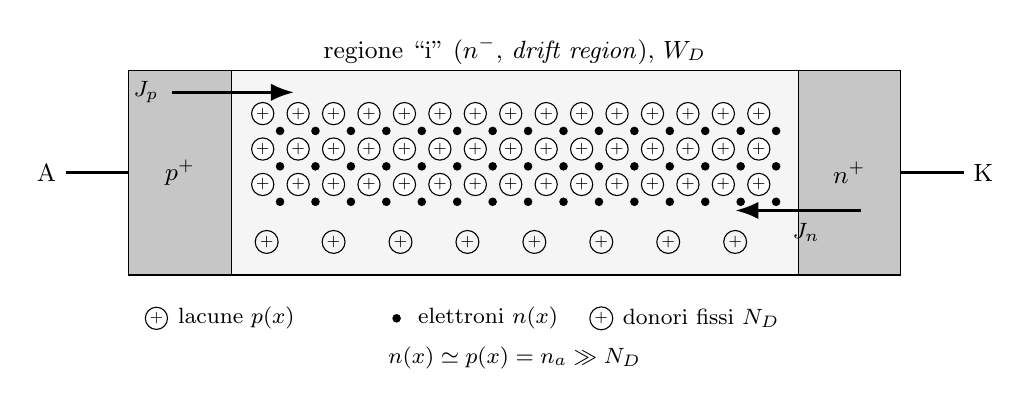
\begin{tikzpicture}[font=\small,>=Latex]
% strati
\fill[gray!45] (0,0) rectangle (1.3,2.6);
\fill[gray!8]  (1.3,0) rectangle (8.5,2.6);
\fill[gray!45] (8.5,0) rectangle (9.8,2.6);
\draw (0,0) rectangle (9.8,2.6);
\draw (1.3,0) -- (1.3,2.6);
\draw (8.5,0) -- (8.5,2.6);
\node at (0.65,1.3) {$p^{+}$};
\node at (9.15,1.3) {$n^{+}$};
\node at (4.9,2.85) {regione ``i'' ($n^{-}$, \emph{drift region}), $W_D$};
% donori fissi
\foreach \x in {1.75,2.6,3.45,4.3,5.15,6.0,6.85,7.7}{
  \node[circle,draw,inner sep=0.6pt,font=\tiny] at (\x,0.42) {$+$};
}

% plasma: lacune (o) ed elettroni (-)
\foreach \x in {1.7,2.15,2.6,3.05,3.5,3.95,4.4,4.85,5.3,5.75,6.2,6.65,7.1,7.55,8.0}{
  \foreach \y in {1.15,1.6,2.05}{
    \node[circle,draw,fill=white,inner sep=0.5pt,font=\tiny] at (\x,\y) {$+$};
    \node[circle,fill=black,inner sep=1.1pt] at (\x+0.22,\y-0.22) {};
  }
}
% legenda plasma
\node[circle,draw,fill=white,inner sep=0.5pt,font=\tiny] at (0.35,-0.55) {$+$};
\node[right,font=\footnotesize] at (0.5,-0.55) {lacune $p(x)$};
\node[circle,fill=black,inner sep=1.1pt] at (3.4,-0.55) {};
\node[right,font=\footnotesize] at (3.55,-0.55) {elettroni $n(x)$};
\node[circle,draw,inner sep=0.6pt,font=\tiny] at (6.0,-0.55) {$+$};
\node[right,font=\footnotesize] at (6.15,-0.55) {donori fissi $N_D$};
\node[font=\footnotesize] at (4.9,-1.05) {$n(x) \simeq p(x) = n_a \gg N_D$};
% frecce di iniezione
\draw[->,very thick] (0.55,2.32) -- (2.1,2.32);
\node[left,font=\footnotesize] at (0.5,2.32) {$J_p$};
\draw[->,very thick] (9.3,0.82) -- (7.7,0.82);
\node[below,font=\footnotesize] at (8.6,0.78) {$J_n$};
% terminali
\draw[very thick] (-0.8,1.3) -- (0,1.3);
\draw[very thick] (9.8,1.3) -- (10.6,1.3);
\node[left] at (-0.8,1.3) {A};
\node[right] at (10.6,1.3) {K};
\end{tikzpicture}
\caption{\emph{Double injection} nella regione ``i''. Le lacune iniettate
dall'anodo sono neutralizzate da un pari numero di elettroni richiamati dal
catodo: il plasma resta elettricamente neutro, ma porta la concentrazione di
\emph{entrambi} i portatori 2--3 ordini di grandezza sopra $N_D$.}
\end{figure}

\begin{figure}[htbp]
\centering
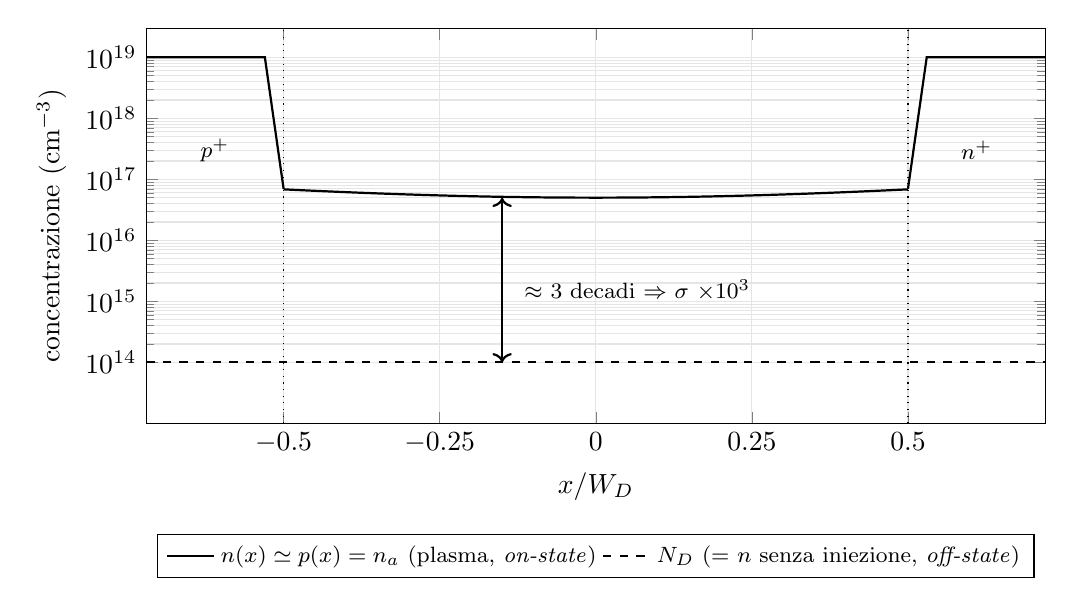
\begin{tikzpicture}
\begin{semilogyaxis}[
  width=13cm, height=6.6cm,
  xlabel={$x/W_D$}, ylabel={concentrazione (\si{\per\centi\meter\cubed})},
  xmin=-0.72, xmax=0.72, ymin=1e13, ymax=3e19,
  xtick={-0.5,-0.25,0,0.25,0.5},
  ytick={1e14,1e15,1e16,1e17,1e18,1e19},
  grid=both, grid style={gray!20},
  legend style={font=\footnotesize,at={(0.5,-0.28)},anchor=north,legend columns=2},
  samples=120,
]
% emitter p+
\addplot[thick,black,forget plot] coordinates {(-0.72,1e19) (-0.53,1e19) (-0.5,7e16)};
% plasma
\addplot[thick,black,domain=-0.5:0.5]
  { 5e16*(exp(x/0.6)+exp(-x/0.6))/(exp(0.833)+exp(-0.833))*1.37 };
\addlegendentry{$n(x) \simeq p(x) = n_a$ (plasma, \emph{on-state})}
% emitter n+
\addplot[thick,black,forget plot] coordinates {(0.5,7e16) (0.53,1e19) (0.72,1e19)};
% ND
\addplot[dashed,thick,domain=-0.72:0.72] {1e14};
\addlegendentry{$N_D$ (= $n$ senza iniezione, \emph{off-state})}
\draw[<->,thick] (axis cs:-0.15,1e14) -- (axis cs:-0.15,5e16);
\node[right,font=\footnotesize] at (axis cs:-0.13,1.5e15)
  {$\approx$ 3 decadi $\Rightarrow$ $\sigma$ $\times 10^{3}$};
\draw[dotted] (axis cs:-0.5,1e13) -- (axis cs:-0.5,3e19);
\draw[dotted] (axis cs:0.5,1e13) -- (axis cs:0.5,3e19);
\node[font=\footnotesize] at (axis cs:-0.61,3e17) {$p^{+}$};
\node[font=\footnotesize] at (axis cs:0.61,3e17) {$n^{+}$};
\end{semilogyaxis}
\end{tikzpicture}
\caption{Profilo delle concentrazioni in scala logaritmica. In blocco la regione
``i'' ha solo $n = N_D$; in conduzione il plasma iniettato porta
$n \simeq p = n_a$ di 2--3 decadi più in alto, con andamento quasi piatto
quando $L_a \gtrsim W_D$.}
\end{figure}

\subsubsection*{Conducibilità e caduta sulla regione modulata}

Poiché conducono \emph{entrambe} le specie, la conducibilità locale vale

\begin{equation}
\sigma(x) = q\left[\mu_n n(x) + \mu_p p(x)\right]
\simeq q\,(\mu_n + \mu_p)\, n_a ,
\end{equation}

da confrontare con il valore in assenza di iniezione
$\sigma_0 = q \mu_n N_D$. Il rapporto è

\begin{equation}
\frac{\sigma}{\sigma_0} = \frac{\mu_n + \mu_p}{\mu_n}\cdot\frac{n_a}{N_D}
\approx 1.35 \cdot \frac{n_a}{N_D} \sim 10^{3} .
\end{equation}

Con l'approssimazione di Mohan di profilo \emph{piatto} (valida se
$L_a \gtrsim W_D$, cioè se la ricombinazione interna è modesta), la carica
immagazzinata è semplicemente

\begin{equation}
Q_F = q A W_D n_a = I_F \tau_{HL}
\quad\Longrightarrow\quad
n_a = \frac{I_F \tau_{HL}}{q A W_D} .
\label{eq:na}
\end{equation}

Sostituendo la \eqref{eq:na} nella caduta ohmica sulla regione modulata si
ottiene il risultato più elegante di questa trattazione:

\begin{equation}
V_{drift} = \frac{I_F W_D}{\sigma A}
= \frac{I_F W_D}{q(\mu_n+\mu_p) n_a A}
= \boxed{\ \frac{W_D^{2}}{(\mu_n + \mu_p)\, \tau_{HL}}\ }
\label{eq:vdrift}
\end{equation}

\noindent
\textbf{cioè una caduta indipendente dalla corrente.} La corrente si
``autoalimenta'' la propria conducibilità: raddoppiando $I_F$ raddoppia anche
$n_a$, e la resistenza si dimezza. La regione ``i'' non si comporta come un
resistore, ma come una piccola caduta quasi costante in serie alla giunzione.

\subsubsection*{Esempio numerico}

Con $W_D = \SI{100}{\micro\meter}$, $N_D = \SI{1e14}{\per\centi\meter\cubed}$,
$\mu_n + \mu_p = \SI{1830}{\centi\meter\squared\per\volt\per\second}$,
$\tau_{HL} = \SI{1}{\micro\second}$, a
$J = \SI{100}{\ampere\per\centi\meter\squared}$:

\begin{table}[htbp]
\centering
\caption{Effetto della \emph{conductivity modulation} sulla regione ``i''.}
\begin{tabular}{lcc}
\toprule
 & senza iniezione & con plasma \\
\midrule
Concentrazione elettroni & $\SI{1e14}{\per\centi\meter\cubed}$ & $n_a \approx \SI{6e16}{\per\centi\meter\cubed}$ \\
Resistenza specifica & $R_{on,sp} = W_D/(q\mu_n N_D) \approx \SI{0.46}{\ohm\centi\meter\squared}$ & --- \\
Caduta sulla regione ``i'' & $\approx \SI{46}{\volt}$ & $W_D^2/[(\mu_n+\mu_p)\tau_{HL}] \approx \SI{55}{\milli\volt}$ \\
\bottomrule
\end{tabular}
\end{table}

Tre ordini di grandezza: è questo che rende utilizzabile una struttura PIN come
diodo di potenza. Senza modulazione, un diodo da \SI{1200}{\volt} avrebbe una
$V_F$ di decine di volt.

\subsubsection*{Limiti dell'approssimazione e prezzo da pagare}

\begin{itemize}
\item La \eqref{eq:vdrift} vale finché il profilo è piatto. Se
$W_D / L_a \gtrsim 2$ il plasma si svuota al centro (Fig.~\ref{fig:catenaria}) e $V_{drift}$
cresce \emph{esponenzialmente} con $W_D/L_a$: per questo un diodo \emph{fast},
con $\tau_{HL}$ ridotto, paga sempre in $V_F$.
\item Sopra $n_a \approx \SI{1e17}{\per\centi\meter\cubed}$ interviene il
\emph{carrier--carrier scattering}: le mobilità calano con $n_a$, $V_{drift}$
riprende a crescere con la corrente e ricompare un comportamento ohmico.
\item A corrente molto alta l'iniezione è limitata dalla ricombinazione negli
\emph{emitter}, quindi $n_a$ cresce meno che linearmente con $I_F$.
\item Soprattutto: la stessa carica $Q_F = I_F \tau_{HL}$ che dà la bassa $V_F$
va \emph{estratta} allo spegnimento. La \eqref{eq:vdrift} e la
$Q_{rr}$ del \S\ref{sec:rr} sono le due facce dello stesso parametro
$\tau_{HL}$: è il compromesso fondamentale del dispositivo bipolare.
\end{itemize}

\subsection{Carica immagazzinata e tensione diretta}

La carica di plasma è

\begin{equation}
Q_F = q A \int_{-d}^{+d} n(x)\,dx \approx I_F \, \tau_{HL} .
\label{eq:QF}
\end{equation}

La \eqref{eq:QF} è la relazione più importante dal punto di vista applicativo:
\emph{la carica da estrarre allo spegnimento è proporzionale alla corrente
condotta e al carrier lifetime}.

La tensione diretta totale si scompone in tre contributi:

\begin{equation}
V_F = \underbrace{V_{j,p^{+}n}}_{\approx \SI{0.7}{\volt}}
+ \underbrace{V_{M}}_{\text{plasma}}
+ \underbrace{V_{j,nn^{+}}}_{\text{piccolo}} ,
\end{equation}

dove $V_M$ è la caduta sulla regione modulata. Nel caso ideale
$W_D \ll L_a$ si trova il celebre risultato

\begin{equation}
V_{M} \approx \frac{3\pi}{8}\,\frac{kT}{q}
\qquad (\approx \SI{30}{\milli\volt}),
\end{equation}

praticamente indipendente dalla corrente: la modulazione della conducibilità è
così efficace da cancellare la resistenza della base. Nella realtà
$W_D / L_a \gtrsim 1$ e $V_M$ cresce esponenzialmente con questo rapporto.

Va aggiunto che a corrente elevata la $V_F$ è limitata dalla ricombinazione
negli \emph{emitter} (\emph{emitter recombination}), descritta da

\begin{equation}
J_{emitter} = q\, h_{p}\, p_{0}^{2},
\end{equation}

dove $h_p$ è il \emph{emitter recombination parameter}. Questo termine è
determinante nel definire la pendenza della caratteristica ad alta corrente.

\subsection{Comportamento in temperatura}

La caratteristica $V_F(I_F)$ presenta un punto di \emph{crossover}:

\begin{itemize}
\item a bassa corrente il coefficiente di temperatura è \textbf{negativo}
(NTC), perché domina la tensione di giunzione, che cala di circa
$-\SI{2}{\milli\volt\per\kelvin}$ per l'aumento di $n_i$;
\item ad alta corrente il coefficiente diventa \textbf{positivo} (PTC), perché
la mobilità cala con $T$ ($\mu \propto T^{-2.4}$) e domina la caduta ohmica sul
plasma e sui \emph{contact layers}.
\end{itemize}

Il comportamento PTC nella zona di lavoro nominale è ciò che rende possibile il
parallelo di più chip o moduli senza \emph{current hogging}: è un criterio di
selezione da verificare sempre sul datasheet quando si mettono in parallelo
diodi.

%======================================================================
\section{Reverse recovery}
\label{sec:rr}
%======================================================================

\subsection{Sequenza fisica}

Allo spegnimento la corrente non può annullarsi istantaneamente: la giunzione
resta polarizzata direttamente finché il plasma è presente. La sequenza,
imposta dal circuito attraverso il $di/dt$ (nella pratica: la velocità di
accensione dell'IGBT o del MOSFET complementare), è la seguente.

\begin{enumerate}
\item \textbf{$t < t_0$}: conduzione, plasma a catenaria, carica $Q_F$.
\item \textbf{Rampa di corrente}: la corrente scende con
$di/dt = -V_{DC}/L_{\sigma}$ (o imposta da $R_g$). Il diodo è ancora
in conduzione, $v_{AK} \approx V_F$: \emph{la giunzione non può ancora bloccare}.
\item \textbf{Attraversamento dello zero e intervallo $t_a$}: la corrente
diventa negativa ed estrae il plasma dal lato $p^{+}$. Finché resta plasma
adiacente alla giunzione, la tensione inversa non può salire. Al termine di
$t_a$ la concentrazione al bordo si annulla, si forma la \emph{space charge
region} e la corrente raggiunge il picco $I_{RM}$ (\emph{peak reverse recovery
current}).
\item \textbf{Intervallo $t_b$}: la \emph{space charge region} si espande, la
tensione inversa sale rapidamente verso $V_{DC}$ (con \emph{overshoot} dovuto a
$L_\sigma\,di/dt$) e la corrente decade a zero man mano che il plasma residuo
viene estratto e ricombinato.
\end{enumerate}

\begin{figure}[htbp]
\centering
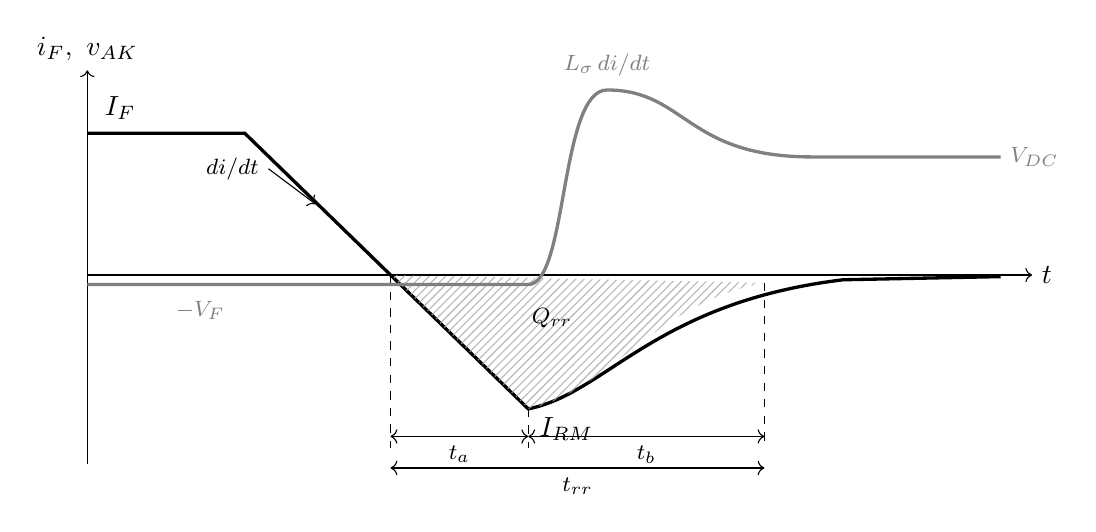
\begin{tikzpicture}[scale=1.0]
% assi
\draw[->] (0,0) -- (12,0) node[right] {$t$};
\draw[->] (0,-2.4) -- (0,2.6) node[above] {$i_F,\ v_{AK}$};
\draw[dashed] (0,0) -- (12,0);
% corrente
\draw[very thick] (0,1.8) -- (2.0,1.8) -- (5.6,-1.7)
   .. controls (6.6,-1.5) and (7.2,-0.35) .. (9.6,-0.06)
   -- (11.6,-0.02);
\node[above right] at (0.1,1.85) {$I_F$};
\node[below right] at (5.62,-1.68) {$I_{RM}$};
% zero crossing e marker
\draw[dashed] (3.85,0) -- (3.85,-2.2);
\draw[dashed] (5.6,-1.7) -- (5.6,-2.2);
\draw[dashed] (8.6,-0.1) -- (8.6,-2.2);
\draw[<->] (3.85,-2.05) -- (5.6,-2.05) node[midway,below] {\footnotesize $t_a$};
\draw[<->] (5.6,-2.05) -- (8.6,-2.05) node[midway,below] {\footnotesize $t_b$};
\draw[<->] (3.85,-2.45) -- (8.6,-2.45) node[midway,below] {\footnotesize $t_{rr}$};
% area Qrr
\fill[pattern=north east lines,pattern color=gray!70,opacity=0.8]
  (3.85,0) -- (5.6,-1.7) .. controls (6.6,-1.5) and (7.2,-0.35) .. (8.6,-0.1) -- cycle;
\node at (5.9,-0.55) {\footnotesize $Q_{rr}$};
% di/dt
\draw[<-] (2.9,0.9) -- (2.3,1.35) node[left] {\footnotesize $di/dt$};
% tensione
\draw[very thick,gray] (0,-0.12) -- (5.6,-0.12)
   .. controls (6.1,-0.12) and (6.0,2.35) .. (6.6,2.35)
   .. controls (7.6,2.35) and (7.6,1.5) .. (9.2,1.5) -- (11.6,1.5);
\node[gray,right] at (11.6,1.5) {\footnotesize $V_{DC}$};
\node[gray,above] at (6.6,2.4) {\footnotesize $L_\sigma\,di/dt$};
\node[gray,right] at (1.0,-0.45) {\footnotesize $-V_F$};
\end{tikzpicture}
\caption{Forme d'onda di \emph{reverse recovery} (comportamento \emph{soft}).
L'area tratteggiata è la \emph{reverse recovery charge} $Q_{rr}$. Un
comportamento \emph{snappy} corrisponde a $t_b \to 0$, con conseguente
sovratensione elevata su $L_\sigma$.}
\end{figure}

\subsection{Grandezze di datasheet e relazioni}

Definendo il \emph{softness factor} $S = t_b/t_a$ e approssimando la forma
d'onda con due segmenti triangolari:

\begin{align}
Q_{rr} &= \tfrac{1}{2} I_{RM} t_{rr}, \\
I_{RM} &= \sqrt{\frac{2\, Q_{rr}\, |di/dt|}{1+S}}, \\
t_{rr} &= \sqrt{\frac{2\, Q_{rr}\, (1+S)}{|di/dt|}}, \\
t_a &= \frac{I_{RM}}{|di/dt|} .
\end{align}

Punti da tenere presenti nel dimensionamento:

\begin{itemize}
\item $Q_{rr} < Q_F$ sempre, perché una parte del plasma ricombina durante
$t_a$; il rapporto è tanto minore quanto più lento è il $di/dt$.
\item $I_{RM} \propto \sqrt{di/dt}$: accelerare la commutazione riduce le
perdite dell'interruttore attivo ma aumenta il picco di \emph{recovery} e le
sovratensioni.
\item Tutte le grandezze crescono con la temperatura, perché $\tau_{HL}$ cresce
con $T$: tipicamente $Q_{rr}$ e $I_{RM}$ raddoppiano fra \SI{25}{\celsius} e
\SI{125}{\celsius}. \textbf{I valori di dimensionamento vanno sempre presi a
$T_{vj,max}$.}
\item L'energia dissipata nel diodo vale
$E_{rec} = \int v_{AK}\, i\, dt \approx Q_{rr} V_{DC} \cdot k$, con $k$ dipendente
dalla forma d'onda ($k \approx 0.5$--$0.8$).
\end{itemize}

\subsection{Soft vs snappy recovery}

Il criterio di scelta più importante, oltre a $Q_{rr}$, è la \emph{softness}. Se
il plasma si esaurisce bruscamente ($t_b \to 0$), la $di/dt$ di coda diventa
molto elevata e l'induttanza parassita genera

\begin{equation}
V_{peak} = V_{DC} + L_{\sigma} \left|\frac{di}{dt}\right|_{tail},
\end{equation}

che può superare la $V_{RRM}$ e distruggere il diodo, oltre a generare EMI e
oscillazioni con la capacità di giunzione. Un diodo \emph{soft} mantiene
plasma residuo verso il lato $n^{+}$ e fa decadere la corrente gradualmente.
Ai fini pratici: la \emph{softness} conta più del valore assoluto di $Q_{rr}$,
soprattutto nei moduli ad alta corrente con $L_\sigma$ non trascurabile.

\subsection{Dynamic avalanche}

Durante $t_b$ coesistono alta tensione ed elevata densità di lacune in transito
nella \emph{space charge region}. Le lacune mobili si sommano alla carica dei
donori:

\begin{equation}
\frac{dE}{dx} = \frac{q}{\varepsilon_{Si}}\left(N_D + p_{drift}\right),
\qquad p_{drift} = \frac{J}{q\, v_{sat}} ,
\end{equation}

aumentando la pendenza del campo e quindi il picco di $E$. Ne consegue che la
capacità di blocco dinamica è inferiore a quella statica: da qui i limiti
$RBSOA$ del diodo e le curve di \emph{safe operating area} in
\emph{reverse recovery} riportate sui datasheet dei moduli.

\subsection{Forward recovery}

Fenomeno duale, spesso trascurato: all'accensione il plasma non è ancora
formato e la \emph{drift region} è ancora resistiva, per cui si osserva un picco
di tensione diretta $V_{FR}$ che può raggiungere decine di volt (in diodi ad
alta tensione anche \SIrange{50}{200}{\volt}) per un tempo $t_{fr}$ dell'ordine
di qualche centinaio di \si{\nano\second}. È rilevante nei convertitori con
$di/dt$ elevato e nei circuiti di \emph{clamping}.

%======================================================================
\section{Tecnologie costruttive}
%======================================================================

Il compromesso fondamentale è $V_F$ contro $Q_{rr}$ (equivalentemente
$E_{rec}$). Le leve disponibili sono le seguenti.

\begin{description}
\item[Lifetime control omogeneo.] Introduzione di centri di ricombinazione:
oro (livello profondo, alta corrente di leakage), platino (livello più
favorevole, migliore compromesso), o irraggiamento con elettroni. Riduce
$\tau_{HL}$ e quindi $Q_{rr}$, ma alza $V_F$ e peggiora il leakage a caldo.

\item[Local lifetime control.] Irraggiamento con elio (He$^{2+}$) o protoni a
profondità controllata, per creare una zona a bassa $\tau$ solo vicino alla
giunzione $p^{+}n^{-}$ (concetto CAL, \emph{Controlled Axial Lifetime}). Si
riduce la carica dove serve, mantenendo il plasma sul lato $n^{+}$: si ottiene
insieme basso $Q_{rr}$ e comportamento \emph{soft}.

\item[Emitter efficiency control.] Riduzione del drogaggio dell'anodo $p^{+}$
per limitare l'iniezione di lacune. Ottimo per la \emph{softness} e per la
robustezza a caldo (concetti \emph{EMCON}, \emph{Emitter Controlled Diode}).

\item[MPS / Merged PiN-Schottky.] Anodo strutturato che alterna zone $p^{+}$ e
contatti Schottky: conduzione bipolare a corrente elevata, unipolare a corrente
bassa, carica immagazzinata fortemente ridotta.

\item[Field stop / buffer.] Consente di ridurre $W_D$ a parità di $V_{BR}$
(quindi meno plasma e minore $V_F$) e impedisce che la \emph{space charge
region} raggiunga l'$n^{+}$ svuotando bruscamente il plasma
(causa tipica di comportamento \emph{snappy}).
\end{description}

\subsection{Confronto con le Schottky in SiC}

Il diodo Schottky in SiC non ha iniezione di minoritari: non esiste plasma da
estrarre, e l'unica carica in gioco è quella capacitiva $Q_C$ della giunzione,
di uno-due ordini di grandezza inferiore a $Q_{rr}$ e \emph{indipendente dalla
temperatura e dal $di/dt$}. Questo elimina il picco $I_{RM}$ e le relative
perdite di \emph{turn-on} nell'interruttore attivo, che nei convertitori
\emph{hard switching} sono spesso il contributo dominante. Il prezzo è il costo
e una minore capacità di sovraccarico ($I^{2}t$) rispetto al PIN in silicio.

\begin{table}[htbp]
\centering
\caption{Confronto qualitativo (valori indicativi, classe \SI{1200}{\volt}).}
\begin{tabular}{lccc}
\toprule
 & Standard Si PIN & Fast/CAL Si PIN & SiC Schottky \\
\midrule
$V_F$ a $I_{nom}$, \SI{25}{\celsius} & \SI{1.1}{\volt} & \SIrange{1.6}{2.0}{\volt} & \SIrange{1.4}{1.8}{\volt} \\
$Q_{rr}$ relativa & 1 & 0.2--0.4 & $<0.05$ \\
Dipendenza da $T$ & forte & forte & trascurabile \\
Dipendenza da $di/dt$ & forte & forte & trascurabile \\
\emph{Softness} & variabile & buona & non applicabile \\
Sovraccarico $I^{2}t$ & ottimo & buono & limitato \\
\bottomrule
\end{tabular}
\end{table}

%======================================================================
\section{Implicazioni a livello di convertitore}
%======================================================================

\begin{itemize}
\item \textbf{Perdite di turn-on dell'interruttore attivo.} Il picco $I_{RM}$
si somma alla corrente di carico mentre la tensione è ancora piena: in un
inverter \emph{hard switching} il contributo del \emph{recovery} può valere
il \SIrange{30}{50}{\percent} di $E_{on}$. Il diodo di \emph{freewheeling}
influenza quindi le perdite dell'IGBT più di quanto non influenzi le proprie.

\item \textbf{Scelta di $R_g$.} Aumentare $R_g$ riduce $di/dt$ e quindi $I_{RM}$
e le sovratensioni, ma allunga la commutazione; il punto di ottimo va cercato
sperimentalmente con misure di \emph{double pulse test}.

\item \textbf{Layout e $L_\sigma$.} Poiché la sovratensione è
$L_\sigma\,di/dt$, il progetto del \emph{DC-link} laminato e la
posizione dei condensatori di \emph{snubber} sono parte integrante del
dimensionamento del diodo.

\item \textbf{Snubber RC/RCD.} Smorzano l'oscillazione fra $L_\sigma$ e la
capacità di giunzione dopo il \emph{recovery}, importante soprattutto con diodi
\emph{snappy} o serie di diodi in alta tensione.

\item \textbf{Serie di diodi.} Con $n$ diodi in serie, le differenze di
$Q_{rr}$ causano ripartizione dinamica non uniforme della tensione: servono
condensatori di \emph{grading} oltre alle resistenze statiche.

\item \textbf{Double pulse test.} È la misura di riferimento per estrarre
$I_{RM}$, $t_{rr}$, $Q_{rr}$, $E_{rec}$ in funzione di $I_F$, $V_{DC}$, $di/dt$
e $T_{vj}$, e per validare i modelli di simulazione.
\end{itemize}

%======================================================================
\section{Riepilogo}
%======================================================================

\begin{table}[htbp]
\centering
\caption{Grandezze principali e loro origine fisica.}
\begin{tabular}{lll}
\toprule
Grandezza & Relazione & Origine fisica \\
\midrule
$V_{bi}$ & $(kT/q)\ln(N_A N_D/n_i^2)$ & allineamento di $E_F$ in equilibrio \\
$np$ & $n_i^2 \exp(qV_j/kT)$ & \emph{splitting} dei quasi-Fermi levels \\
$W_D$ & $\sqrt{2\varepsilon V_{BR}/(qN_D)}$ & campo critico $E_c$ \\
$n(x)$ & catenaria, \eqref{eq:catenaria} & \emph{ambipolar diffusion equation} \\
$Q_F$ & $I_F \tau_{HL}$ & plasma immagazzinato \\
$I_{RM}$ & $\sqrt{2 Q_{rr} (di/dt)/(1+S)}$ & estrazione del plasma \\
$E_{rec}$ & $\approx k\, Q_{rr} V_{DC}$ & sovrapposizione $v$--$i$ \\
$V_{peak}$ & $V_{DC} + L_\sigma (di/dt)_{tail}$ & \emph{snappiness} + parassiti \\
\bottomrule
\end{tabular}
\end{table}

Il messaggio di sintesi è che il \emph{power diode} PIN è un dispositivo
governato da un unico compromesso, la quantità di plasma nella
\emph{drift region}: molto plasma significa bassa $V_F$ e alte perdite di
commutazione, poco plasma il contrario. Tutte le tecnologie moderne
(\emph{local lifetime control}, \emph{emitter efficiency control}, MPS,
\emph{field stop}) non fanno altro che ridistribuire il plasma nello spazio
invece di ridurlo uniformemente, per ottenere insieme basso $Q_{rr}$ e
comportamento \emph{soft}.

%======================================================================
\begin{thebibliography}{9}

\bibitem{baliga}
B.~J. Baliga, \emph{Fundamentals of Power Semiconductor Devices}, 2nd ed.
Cham, Switzerland: Springer, 2019.

\bibitem{lutz}
J.~Lutz, H.~Schlangenotto, U.~Scheuermann, and R.~De Doncker,
\emph{Semiconductor Power Devices: Physics, Characteristics, Reliability},
2nd ed. Cham, Switzerland: Springer, 2018.

\bibitem{mohan}
N.~Mohan, T.~M. Undeland, and W.~P. Robbins, \emph{Power Electronics:
Converters, Applications, and Design}, 3rd ed. Hoboken, NJ, USA: Wiley, 2003,
ch.~20.

\bibitem{sze}
S.~M. Sze and K.~K. Ng, \emph{Physics of Semiconductor Devices}, 3rd ed.
Hoboken, NJ, USA: Wiley, 2007.

\bibitem{hall}
R.~N. Hall, ``Power rectifiers and transistors,''
\emph{Proc. IRE}, vol.~40, no.~11, pp.~1512--1518, Nov. 1952.

\bibitem{lauritzen}
P.~O. Lauritzen and C.~L. Ma, ``A simple diode model with reverse recovery,''
\emph{IEEE Trans. Power Electron.}, vol.~6, no.~2, pp.~188--191, Apr. 1991.

\bibitem{cal}
J.~Lutz and W.~Sudkamp, ``The CAL diode --- a fast, soft and rugged diode,''
in \emph{Proc. EPE}, Trondheim, Norway, 1997.

\bibitem{scheuermann}
U.~Scheuermann and R.~Schmidt, ``Impact of load pulse duration on power cycling
lifetime of Al wire bonds,'' \emph{Microelectron. Rel.}, vol.~53, 2013.

\bibitem{infineon}
Infineon Technologies, \emph{Application Note AN2015-11: Power Semiconductor
Switching Losses and Diode Reverse Recovery}, 2015.

\end{thebibliography}

\end{document}
